\subsection{Why the O(I) vacancy?}


\subsubsection{Total density of states}

Notice the new level in the band gap - defect level - filled.

\begin{figure}[H]
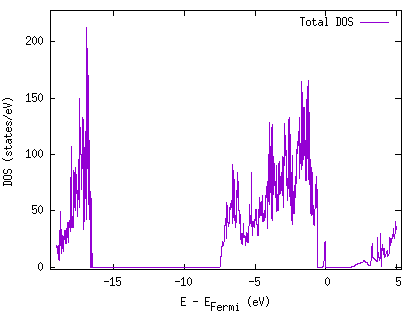
\includegraphics[width=\linewidth]{../fig/dosplot/total_dos_O_I_vacancy}\caption{This is a plot of the density of state of the super cell with a O(I) vacancy.}\label{fig:total_dos_vac}
\end{figure}

\begin{figure}[H]
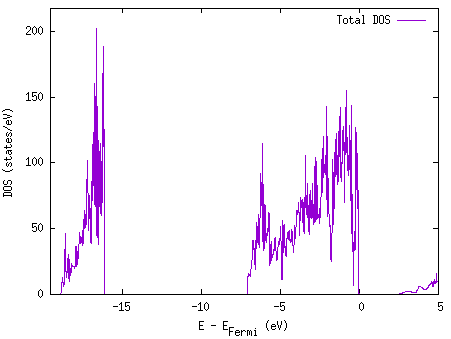
\includegraphics[width=\linewidth]{../fig/dosplot/total_dos_supercell}\caption{This is a plot of density of state of the general supercell.}\label{fig:total_dos_supercell}
\end{figure}

\subsubsection{Isosurfaces}

Figure \ref{fig:isosurface_O_I} shows the structure around the O(I) vacancy with different electron density isosurface levels. When the isosurface level is set to 0.04, an electron density is visible between the two Ga(I) atoms the O(I) atom should have been bonded to and and when the isosurface level is 0.03, the isosurface shows a bond between them (Figure \ref{fig:bond_O_I}).

\begin{figure}[H]
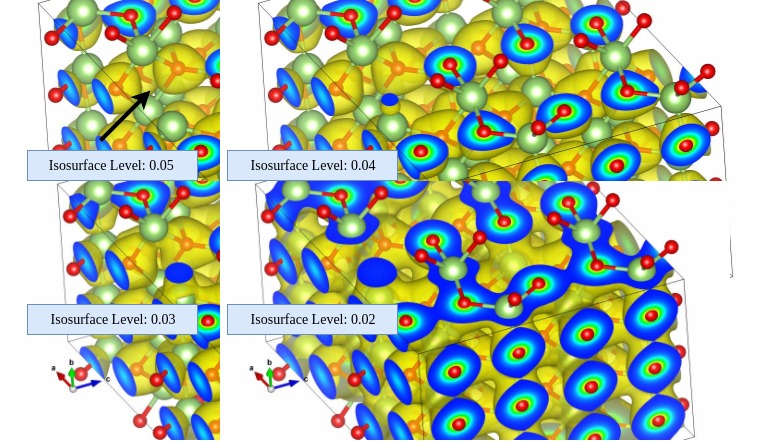
\includegraphics[width=0.9\linewidth]{../fig/isosurfaces/O_I/isosurface}\caption{This figure shows the O(I) vacancy with different electron density isosurfaces.The black arrow points to the O(I) vacancy. When the isosurface level is lowered, a bond appears between the two Ga(I) atoms the O(I) should have been bonded to (Figure \ref{fig:bond_O_I}).}\label{fig:isosurface_O_I}
\end{figure}

\begin{figure}[H]
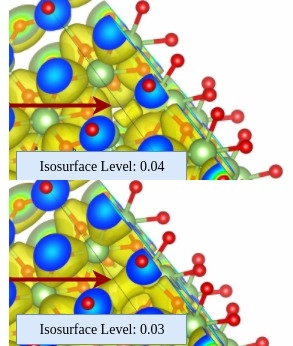
\includegraphics[width=0.7\linewidth]{../fig/isosurfaces/O_I/bond}\caption{This figure shows the oxygen vacancy with different isosurfaces.In this figure the bond between the two Ga(I) atoms shows clearly. The isosurface goes from one atom to the other at the isosurface level 0.03.}\label{fig:bond_O_I}
\end{figure}

Figure \ref{fig:isosurface_O_II} shows the O(II) vacancy with different isosurfaces, when the isosurface level is lowered, the electron density around the Ga(I)-atom shows. The 'blob' shows the dangling bonds at the Ga(I) atom, but there is no 'blob' at the Ga(II) atoms. With the O(II) vacancy the isosurface level needs to be 0.02 for there to be a connection with the other Ga(II) atoms.

\begin{figure}[H]
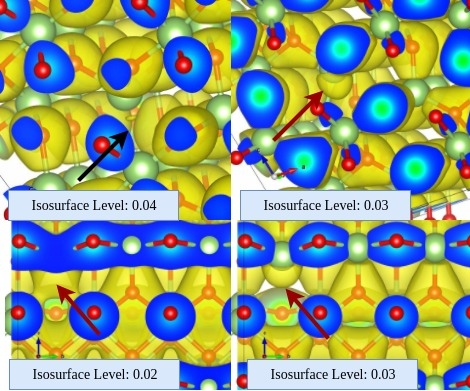
\includegraphics[width=\linewidth]{../fig/isosurfaces/O_II/isosurface}\caption{This figure shows the O(II) vacancy with different electron density isosurfaces.The figure shows the oxygen vacancy from different angles. The black arrow points to the vacancy and the red arrows points to the isosurface indicating dangling bonds at the Ga(I) atom.}\label{fig:isosurface_O_II}
\end{figure}

Figure \ref{fig:isosurface_O_III} shows the same for the O(III) vacancy. As in the case for the O(II) vacancy, the isosurface level needs to be 0.02 before there is a connection, and before that there is the same 'blob' at the one Ga(I) atom, indication dangling bonds.

\begin{figure}[H]
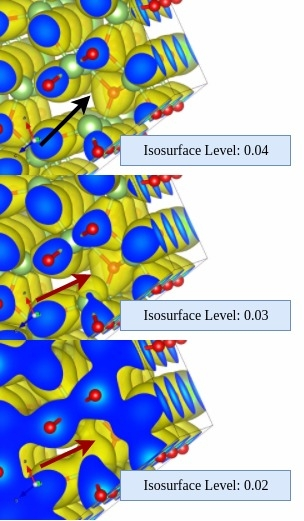
\includegraphics[width=0.7\linewidth]{../fig/isosurfaces/O_III/isosurface}\caption{This figure shows the oxygen vacancy with different electron density isosurfaces.The black arrow points to the oxygen vacancy and the red arrows points to the dangling bond at the Ga(I) atom.}\label{fig:isosurface_O_III}
\end{figure}

The difference between the O(I) vacancy with two Ga(I) atoms, that seems to form a covalent bond in the absence of an oxygen, and the other two vacancies, that only have one Ga(I) atom, might be a reason why the O(I) vacancy has the lowest formation energy.

The reason for the bond between two the Ga(I) atoms may come from the shorter length of the O-Ga(I) bond compared to the O-Ga(II) bond (see Figure \ref{fig:distances}). The 'bulb' from the isosurface always occur at the Ga(I) atom, and nothing at the Ga(II) atoms. Maybe the Ga(I) atom has dangling bonds, and the Ga(II) relocate the electrons elsewhere - is that possible? \ref.

\subsubsection{Local DOS Ga(II)}

\begin{figure}[H]
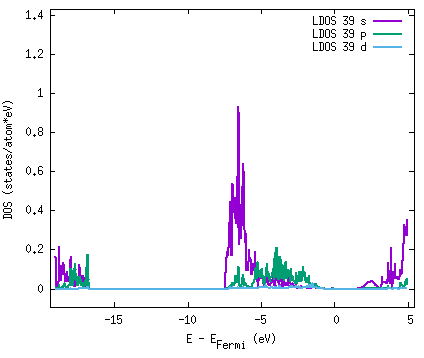
\includegraphics[width=\linewidth]{../fig/dosplot/ldos_Ga_II_OI_vac_nabo}\caption{This is a plot of local density of state at the Ga(II) site next to the O(I) vacancy in the super cell.}\label{fig:ldos_Ga_II_nabo}
\end{figure}

\begin{figure}[H]
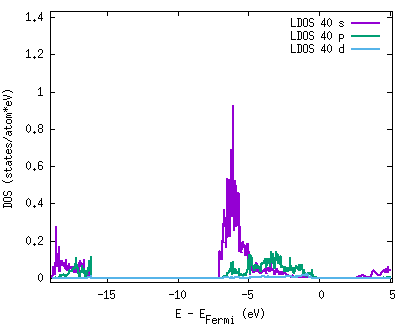
\includegraphics[width=\linewidth]{../fig/dosplot/ldos_Ga_II_supercell}\caption{This is a plot of local density of state at the Ga(II) site in the general supercell.}\label{fig:ldos_Ga_II_supercell}
\end{figure}

\subsubsection{Local DOS Ga(I)$_1$}

\begin{figure}[H]
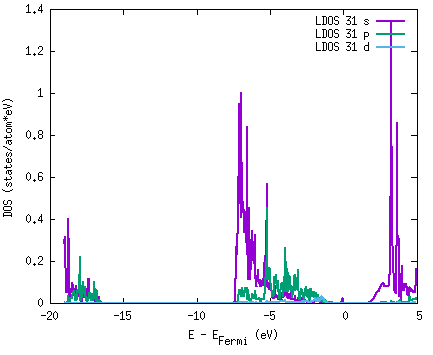
\includegraphics[width=\linewidth]{../fig/dosplot/ldos_Ga_I_OI_vac_nabo}\caption{This is a plot of local density of state at the Ga(I) site next to the O(I) vacancy in the super cell.}\label{fig:ldos_Ga_I_nabo}
\end{figure}

\begin{figure}[H]
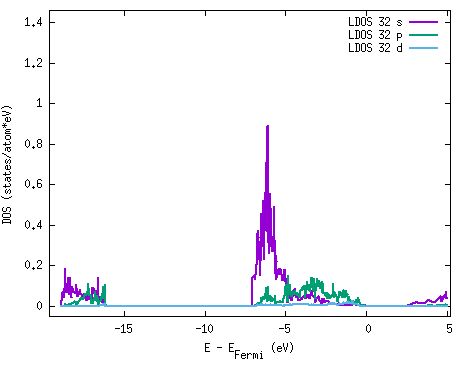
\includegraphics[width=\linewidth]{../fig/dosplot/ldos_Ga_I_supercell}\caption{This is a plot of local density of state at the Ga(I) site in the general supercell.}\label{fig:ldos_Ga_I_supercell}
\end{figure}

\subsubsection{Bond between Ga(I)$_1$ and Ga(I)$_2$?}

\begin{figure}[H]
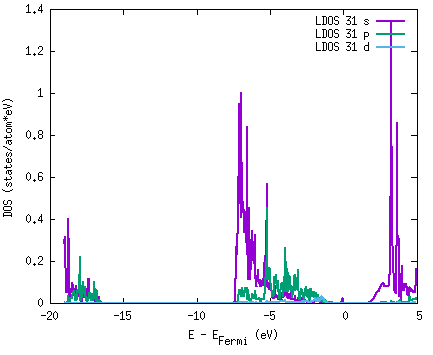
\includegraphics[width=\linewidth]{../fig/dosplot/ldos_Ga_I_OI_vac_nabo}\caption{This is a plot of local density of state at the Ga(I) site next to the O(I) vacancy in the super cell.}\label{fig:ldos_Ga_I_nabo}
\end{figure}

\begin{figure}[H]
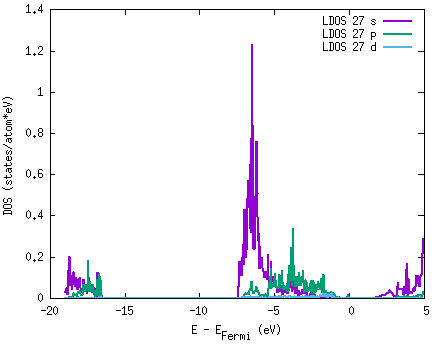
\includegraphics[width=\linewidth]{../fig/dosplot/ldos_Ga_I_OI_vac_nabo2}\caption{This is a plot of local density of state at the other Ga(I) site next to the O(I) vacancy in the super cell.}\label{fig:ldos_Ga_I_nabo}
\end{figure}
